%\documentclass[sigconf]{acmart}
\documentclass{article}
\usepackage[margin=1.8in]{geometry}

\usepackage[]{graphicx}
\usepackage[]{color}
\usepackage{subfig}
\usepackage{listings}
\usepackage{url}

%\usepackage{alltt}
\usepackage{multicol}
%\pagestyle{plain}
%\usepackage{amsmath}
%\usepackage{caption} 
%\captionsetup[table]{skip=3pt}

\begin{document}

\title{DetGen: How to make traffic generation and monitoring at packet level more dynamic using containerisation}
%Dynamic Traffic Generation with Containerization for Machine Learning}

\maketitle

\section{Introduction}

Data-driven traffic analysis and attack detection is a centrepiece of network intrusion detection research, as well as many other fields \textcolor{red}{citations}. Realistic network traffic datasets allow engineers to build a better understanding of existing structures, motivate design choices from actual needs, and prove that proposed new systems can indeed work in practice. \textcolor{red}{something to emphasise that packet traffic is important.}

Unfortunately, privacy and security concerns discourage network administrators to release rich and realistic datasets for the public,  leading to publicly available real-world datasets being the exception and missing informative features such as captured packets or consistent IP-addresses. As a result, researchers are predominantly relying on synthetically generated data, which is currently either captured using scripted activities in a virtual or lab-environment, or generated using trained generative models of real-world traffic.

Existing network intrusion detection datasets are however collected in a static manner, unable to be modified, updated, or reproduced, \textcolor{red}{citation} and therefore can neither adapt to novel attacks or traffic evolutions, nor give researchers the flexibility to focus on particular traffic types. Furthermore, the current capture setups provide no insight in the data generation process, and it is mostly impossible to match events on the packet-level with conducted activities due to the capture setup. 
Existing testbeds and traffic generation frameworks are successful at emulating large-scale traffic characteristics \textcolor{red}{citations}, but fail to provide the necessary detail and realism for intrusion detection on a packet-level. 

%This proves to be a serious defect as the ecosystem of intrusions is continually evolving.
%Furthermore, it prohibits a more detailed analysis of specific areas of network traffic due to the available data only being a fraction of the original dataset. To combat this, new datasets must be periodically built from scratch.


%Furthermore, VM-based traffic simulation frameworks provide little insight into the ...


%Allowing researchers to create datasets dynamically to circumvent these issues would be extremely beneficial. 
We propose a novel design paradigm that makes generation of network traffic and corresponding attacks significantly more flexible and offers a \textcolor{red}{new level} of insight and reproducibility for traffic micro-structures through the use of containerisation. By moving from virtual machines to containers, we enable the scalable, modular, and dynamic creation of network traffic datasets. Since containers can be arranged in complex settings with a few commands, it is a lot easier with containers to script a variety of network activities thus increase the heterogeneity and realism of the generated data.

%Furthermore, each Docker container is highly specialized in its purpose, generating traffic related to only a single application process. Therefore, by scripting a variety of Docker-based \emph{scenarios} that simulate benign or malicious behaviours and collecting the resultant traffic, we can build a dataset with perfect ground truth, something that has so far not been possible for network traffic. 


This work provides the following contributions:

\begin{enumerate}
\item We present a novel network traffic generation framework called \textit{DetGen} that is designed to improve several shortcomings of current datasets and data generation frameworks for NIDS evaluation in the following aspects:
\begin{enumerate}
\item Ground truth labels documenting every conducted activities
\item Increased structural realism of the data on a packet-level
\item Tunable topology, traffic composition, and attack types
\item Capture of program logs and system calls for data fusion methods
\end{enumerate}
This framework is openly accessible for researchers and allows for straightforward customization.
 
%\item We define four new requirements a network intrusion dataset should fulfil in order to be suitable to train machine-learning based intrusion detection methods. 
 %\item how to build new modules that can be added to the existing framework, and how this procedure enables data generation that is more suitable for data-driven methods than currently available datasets.
\item We perform a number of experiments to demonstrate the fidelity to realism of the generated data.
\item We present a number of use-cases to demonstrate how the design of our framework can boost performance for ML-based network intrusion detection systems, in particular for false-positive analysis and effective model training.
\end{enumerate}

%\subsection{Contributions}

%\subsubsection{Main contributions}


%
%\begin{enumerate}
%\item Fidelity to real traffic
%\begin{itemize}
%	\item Real traffic, consistent (not invalid after Cordero et al.)
%	\item Structural richness on packet level (in contrast to )
%		Induced due to the different levels at which traffic variation is introduced
%%	\item Temporal activity levels? (actually not something we improve)
%%			We can look at test for realism of distributions (IP discovery, etc)
%\end{itemize}
%\item Ground truth labels through containerisation
%\begin{itemize}
%	\item Ground truth for attack behaviour, able to label 100\% of the generated events to specific activities
%	\item Labels for different types of behaviour, reproducable
%		useful for evaluation of model failures, what kind of behaviours cause failure
%			applies to a large range of models
%		also useful for evaluation of privacy infiltration methods, more niche
%	\item Ground truth for label matching between traffic and program logs/sys logs
%		useful for models that try to correlate events for detection
%			this is more niche, but potentially because of the lack of data
%\end{itemize}
%\item Extensive capture
%\begin{itemize}
%	\item Packet availability
%	\item Syslogs and for multiple scenarios program logs
%	\item Potentially host logs? Depends if we want to cater to cloud computing applicability
%\end{itemize}
%\item Better for ML-based methods
%\begin{itemize}
%	\item Flexibility 
%		"The models should allow researchers to generate different classes of data, such as augmenting the amount of data representing sparse events, or choose different topology"
%	\item Automisation of variable datasets through randomisation, automatically create structurally different datasets, but faithful to realism
%		Especially novel in terms of network topologies, should emphasise this in use-cases
%	\item Structural richness 
%			allows for learning deeper and more generalisable knowledge in models, less prone to overfitting
%	\item Scalability
%		"Train on as much data as necessary"
%\end{itemize}
%
%\end{enumerate}





\subsection{Outline}

%The remainder of the paper is organized as follows. Section \ref{Sec:background} discusses existing NIDS datasets and the problems that arise during their usage as well as background information about network traffic data formats and virtualization methods. The section concludes with a set of requirements we propose to improve the training and evaluation of machine-learning-based methods. Section \ref{Sec:Design} describes the general design of our framework, and how it improves on the discussed problems in existing datasets. We also discuss a specific example in detail. Section \ref{Sec:Experiments} discusses several experiments to validate the improvements and utility our framework provides. 
%Section \ref{Sec:Conclusion} concludes the results and discusses limitations of our work and directions for future work.

Outline of the coming sections.

\dots \dots

\dots \dots

\dots \dots

\section{Goals and motivation}

If we are to create \textit{realistic} and \textit{reproducible} \textcolor{red}{intrusion detection} experiments, then we need a platform with the following characteristics:

\paragraph{Traffic realism and reproducibility} The system should generate real, interactive network traffic that resembles common traffic structures on a packet-level. The system should make it easy for researchers to verify results by enabling the duplication and running of network intrusion detection systems that are deployed within the platform.   

\paragraph{Ground truth} Activities generating traffic events should run in a reproducible manner to allow replication of traffic traces. Researchers should be able to trace the origin of traffic events to the \textcolor{red}{precise} generating activity.

\paragraph{Flexibility} It should be easy to tune the composition of the generated. Similarly, it should be easy to create an experiment with any topology.

\paragraph{Attack diversity} Intrusion detection models are dependent on attack data that represent specific attacks. The platform should therefore enable the execution or addition of a wide variety of attacks.

%\textbf{Functional realism} The system must have the same functionality as real hardware in a real deployment, and shouldexecute exactly the same code.

\paragraph{Low cost} \textcolor{red}{It should be inexpensive to duplicate an experiment, e.g. for students in a course.}


\vspace{0.3cm}

Table \ref{Tab:Contributions} compares how well existing methods are realising these goals compared to our framework.


Currently, intrusion detection researchers predominantly rely on public, synthetically generated datasets, on which NID systems are evaluated subsequently.
\textit{Real-world datasets} such as LANL-15 \cite{kent-2015-cyberdata1} or UGR-16 \cite{macia2018ugr} provide the highest amount of traffic realism, but often lack detailed information such as packet captures due to privacy reasons, and give close to no information on the content of the provided data. 

\textit{Synthetic datasets} such as the CICIDS-17 \cite{sharafaldin2018towards} or the UNSW-16  \cite{moustafa2015unsw} datasets are typically captured in virtual environments that simulate \textcolor{red}{commercial} networks with virtual machines. Traffic is generated from scripted activity, and attack data either injected or generated from carefully inserted vulnerabilities. The arranged settings normally lack the flexibility to generate customized data and by design only provide very limited attack diversity.
%limited insights into the given traffic realism or 

\textit{Attack traffic generators} typically aim at providing traces from a diverse set of attacks, and injecting them into existing traffic captures in various ways. Moirai \textcolor{red}{citation} for example calculates several quantitative characteristics to better embed the attack traffic.  However, most of the issues surrounding real-world traffic captures remain, and there is concern about the realism of injected attack traffic \textcolor{red}{citation}.

Recently, some effort have been made to to generate completely artificial traffic data with \textit{generative adversarial networks} (GANs) trained on real-world traffic. While examples such as DoppelGANger or Ring et al. \textcolor{red}{citation} are successful at generating realistic large-scale network features such as activity levels or \textcolor{red}{connection graphs}, they are not aimed at intrusion detection and do not provide the necessary granularity to model connection- or packet-level features.

 \textit{Testbeds} such as Mininet offer tremendous \textcolor{red}{flexibility}, but are so far not targeted for intrusion detection and lack suitable small-scale traffic generation tools, labelling capabilities, or attack scenarios. 

\subsection{Motivation \textcolor{red}{(or Use-cases?)}}

While there are many potential use-cases that can benefit from a system like DetGen, we highlight two key types of interactions and three representative tasks in these cases: 

\paragraph{Data-driven tasks}:
\begin{itemize}

\item \textit{In-depth model evaluation}:
Drawing on the extensive labelling of granular activities and reproducible traffic generation, researchers have new opportunities to examine the performance of an intrusion detection model in-depth. Packet-level structures and resulting false-positives can be better associated with activities, which helps correct models better for identified weaknesses. Granular activities can be studied in a less noisy environment due to isolation and reproducibility. 


\item \textit{Boost performance of ML-based methods}: Similarly, the performance of machine-learning-based methods can be boosted by tuning the composition of training data. Datasets can include traffic from different setups (topology, host activities, etc.) to allow for a better model generalization.

\item \textit{Focus on novel attacks and traffic types}: Instead of being restricted to a restricted set of attacks and traffic types, researchers using DetGen can easily embed novel attacks such as the eternal blue exploit or new traffic types such as QUIC in a given network setup without abandoning the overall \textcolor{red}{network coherence} of the data. 


\end{itemize}

\paragraph{\textcolor{red}{Collaborative} tasks}: 

\begin{itemize}
\item \textit{Simulation of deployment}: Instead of evaluating an intrusion detection model subsequently on previously captured data, researchers can deploy their system directly in DetGen to assess issues such as computational speed or \textcolor{red}{...}.



\item \textit{Reproducible, open research}: Scientific experiments should be reproduced to be considered valid, and the use of containers has recently been \textcolor{red}{promoted} to enable easy reproduction of computational work by reducing the need for plattform and library dependencies. Network researchers can use DetGen to allow for the easy reproduction of generated network settings, generated data, and deployed network intrusion solutions. 


\end{itemize}

\begin{table}
\centering
\begin{tabular}{p{3cm}|p{3cm}|p{3cm}|p{2cm}|p{2cm}}
Contribution&How containers enable it& VM-based & Real traffic capture &Other framework  \\ \hline

Ground truth labels on granular activities & Isolated process in container, no additional events. Easy to separate even when containers attached to same network interface & background events (system activitiy, artifacts from earlier activity, ...), overlaying activities hard to separate & No knowledge about conducted activity & Technically possible, no attempts yet \\ \hline

Flexibility to regenerate customized datasets & Launching a network of containers is easy, modularity allows finer control of fine-grain activity  & Difficult to regenerate data as set-up and launching of VM is less straightforward, might be addressed with MiniMega & No & Yes \\ \hline

Easy to update, include new attacks & 
Attack/victim containers remove dependence on vulnerabilities, can be hooked to existing scenarios with shared resources & Since attacks happen on the VM, it is very hard to compose a VM with enough vulnerabilities to include many attacks & - & Some work has been done to "replay" or artificially inject attacks  \\ \hline

Reproducability & Container state the same after repeated launches, isolation means that other task have little effect on, plattform independence  & To a lesser degree, simultaneously conducted activity can affect each other & - & Depends \\ \hline

Fidelity to real traffic heterogeneity, structural richness & Not a lot except that scripting and randomising different scenarios is slightly easier  & Potentially, but little attention has been paid & Yes & Not on a packet level yet \\ \hline \hline


Data on attacks on container isolation & In need of existing scenarios for background data & No & No & No \\ \hline
\end{tabular}
\caption{Contributions compared to existing solutions}\label{Tab:Contributions}
\end{table}


\section{DetGen Architecture}

DetGen is a container-based emulator that we developed to enable repeatable, realistic, and flexible network experiments. DetGen extends the widely-used Mininet testbed \textcolor{red}{insert citation} by adding scenarios for benign and attack traffic generation, event labelling, and p

%\section{Background}\label{Sec:b8ackground}

\subsection{Design overview}

The Detgen framework uses Mininet to create a network with a \textcolor{red}{desired} topology, along with virtual software switches, Ethernet links, routers, and firewalls. The network is then populated with containers ,which perform a variety of activities for traffic generation. The conducted activities are composed of scripted \textit{scenarios} (\textcolor{red}{give examples here}), but subject to a high degree of randomisation. The captured traffic events are labelled individually after the specific generating action. 

\subsection{Containerization}
%\textcolor{red}{to do:need to improve}
Containers are standalone packages that contain an application along with all necessary dependencies using OS-level virtualization. In contrast with standard Virtual machines (VMs), containers forego a hypervisor and the shared resources are instead kernel artifacts that can be shared simultaneously across several containers, leading to minimal CPU, memory, and networking overhead \cite{kolyshkin2006virtualization}.


%\textcolor{red}{Although this prevents the host environment from running different operating systems, containerization incurs minimal CPU, memory, and networking overhead whilst maintaining a great deal of isolation} \cite{kolyshkin2006virtualization}. 

Due to the separation of processes, containers provide significantly more isolation of programs from external effects than regular OS-level execution. This isolation enables us to monitor processes better and create more accurate links between traffic events and individual activities than on a virtual machine were multiple processes run in parallel, which can all generate traffic. The one-to-one correlation between containers and network traces allows us to produce labelled datasets with fully granular ground truths. 

Containers are specified in an image-layer, which is unaffected during the container execution.
This allows containers to be run repeatedly whilst always starting from an identical state. In combination with the container isolation, this allows us to perform network experiments that can be easily reproduced by anyone on any plattform \textcolor{red}{insert citation}. 


The container network interface provides the connection between a network namespace and the container runtimes. We want to \textcolor{red}{highlight} that multiple containers can share on network interface, which enables us to generate traffic from multiple applications over one network address in order to emulate \textcolor{red}{fully functional network hosts}.
 

\subsection{Scenario scripting}\label{Sec:Scenarios}

We define a \emph{scenario} as a series of Docker containers conducting a specific interaction, whereby all resulting network traffic is captured from each container's perspective. This constructs network datasets with total interaction capture, as described by Shiravi et al. \cite{shiravi2012toward}. Each scenario produces traffic from either a protocol, application or a series thereof. %Both benign and malicious activities are implemented as scenarios. 
Examples may include an FTP interaction, a music streaming application and client, an online login form paired with an SQL database, or a C\&C server communicating with an open backdoor. A full list of currently implemented scenarios can be found in Section \ref{Sec:ExistScen}.
Each scenario is designed to be easily started via a single script and can be repeated indefinitely without further instructions, therefore allowing the generation of large amounts of data.

Our framework is modular, so that individual scenarios are configured, stored, and launched independently. Adding or reconfiguring a scenario has no effect on the remaining framework.

\subsubsection*{Subscenarios} \label{Sec:Subscenarios}

In contrast to scenarios, \textit{subscenarios} provide a finer grain of control over the traffic to be generated, allowing the user to specify the manner in which a scenario should develop. The aim of having multiple subscenarios for each scenario is to explore the full breadth of a protocol or application's possible traffic behavior. For instance, the SSH protocol can be used to access the servers console, to retrieve or send files, or for port forwarding, all of which may or may not be successful. It is therefore appropriate to script multiple subscenarios that cover this range of tasks.

%Subscenarios are specific to particular scenarios and can be specified when launching that scenario.

%The same applies to malicious activity. For instance, it would be naive for an SSH password bruteforcing scenario to always successfully guess a user's password. Instead, we include a second subscenario in which the password bruteforcer fails.

\subsubsection*{Randomization within Subscenarios}\label{Sec:randomsubscen}

Scripting activities that are otherwise conducted by human operators often leads to a loss of random variation that is normally inherent to the activity.
\textcolor{red}{As mentioned in Section \ref{Sec:problems}, the majority of successful FTP transfers in the CIC-IDS 2017 data consist of a client downloading a single text file.} In reality, file sizes, log-in credentials, and many other variables included in an activity are more or less drawn randomly, which naturally influences traffic quantities such as packet sizes or numbers.

We identify variable input parameters within scenarios and their subscenarios and systematically draw them randomly from suitable distributions. Passwords and usernames, for instance, are generated as a random sequence of letters with a length drawn from a Cauchy distribution, before they are passed to the corresponding container. Files to be transmitted are selected at random from a larger set of files, covering different sizes and file names.

\begin{figure}
 \centering 
 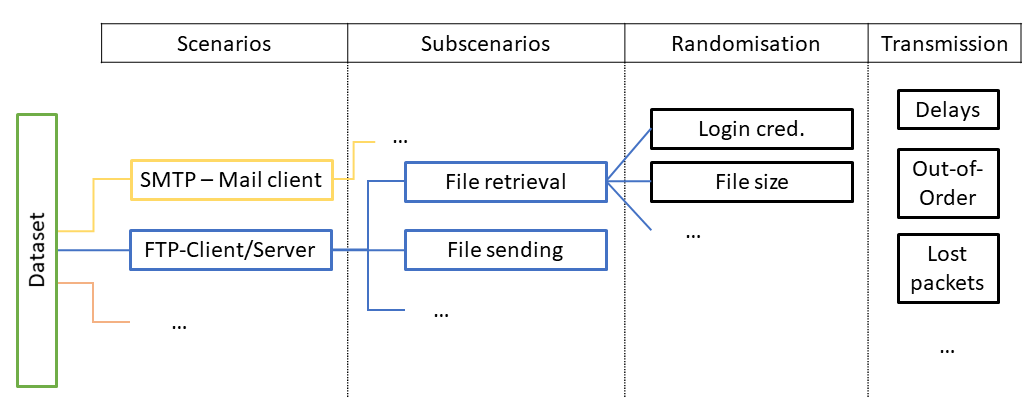
\includegraphics[width=0.480\textwidth]{images/scenario_branching.PNG}
 \caption{Visualization of the different levels at which traffic variation is introduced in DetGen.}
 \label{Fig:branching}
\end{figure}

\subsubsection*{Implementation process}

\subsection{Network creation and population}


To enable communication between containers, we build our framework on top Mininet \textcolor{red}{insert citation} to create virtual networks with customizable topology. 
\textcolor{red}{A topology can be passed to a topology-creation wrapper in matrix form, with diagonal values representing the type of device (switch, container, router, ...), and off-diagonal indicating links}. This allows the import of larger, automatically generated topologies from tools such as \textcolor{red}{insert citation}. 

\textcolor{red}{maybe something about subnets}. 

\subsubsection*{Import of activity timeline}

The modelling and generation of computer network activity has been investigated extensively \textcolor{red}{(citations?)}, and tools to automatically generate realistic network activity streams 

we do not wish to \textcolor{red}{address} this topic here . Instead, our framework imports existing time-series of \textcolor{red}{host flow activity} to generate the corresponding communication. \textcolor{red}{give more info on flow generation tools} 

We transform existing network flow series into an activity timeline by \textcolor{red}{expand this}. We end up with an activity timeline that contains a set of timestamps along with the corresponding scenario and the source and destination host. 

\subsubsection*{Activity conduction}


\subsubsection*{Attack traffic generation}
%\subsubsection{Metasploit and Metasploitable containers}

A description of the capabilities and limitations of both metasploit and the metasploitable VM and the corresponding containers, which we will use.


%\section{Dataset Requirements}\label{Sec:require}

%We can refer to requirements by Cordero et al. (https://arxiv.org/pdf/1905.00304.pdf) on requirements for generating synthetic datasets, and combine them with the existing set of requirements by us. 

%These include:



\subsection{Benefits resulting from design choices}





%In particular, Ring et al. have proposed a method to generate realistic network-wide flow-based traffic that models typical host activity levels. 












\subsection{Related work and existing datasets}

%A similar description on existing frameworks and datasets as in the existing paper, with a slightly higher focus on existing testbeds and existing container tools.
%\dots \dots
%\dots \dots
%\dots \dots

%\subsubsection{Datasets}
%
%real:
%Los Alamos National Laboratory (LANL)
%University of Granada (UGR)
%
%SANTA
%Only flows, manually labelled
%
%
%CAIDA 2016
%
%MAWI 2000
%
%LITNET
%
%synthetic:
%
%CICIDS-17
%UNSB-16
%
%CIDDS-001
%Python scripts are used for emulating benign user behaviour like browsing the web, sending and receiving emails, as well as exchanging files. To ensure as realistic user behaviour as possible, clients perform their activities with respect to an individual working schedule which considers working hours and lunch breaks.
%
%NGIDS-DS
%Uses IXIA Perfect Storm, also collects host logs
%
%
%
%frameworks:
%
%FLAME
%ID2T
%Use real traffic as input to add attack traffic
%GEN-ESIDS
%HTTP attack traffic after user-based attack description
%NDSec-1 - Also overlaying normal data with attack traffic
%
%Moirai
%
%
%A flow trace generator using graph-based traffic classification techniques
%extractstraffictemplatesfromrealnetworktraf-fic.Then,theirgeneratorusesthesetraffictemplatesinordertocreatenewsyntheticflow-basednetworktraffic
%
%INSECS-DCS
%
%
%
%
%Flow-based network traffic generation using Generative Adversarial Networks
%DoppelGANger
%
%weak:
%PACGAN
%PCAPGAN
%SynGAN
%
%
%surveys:
%A Taxonomy of Network Threats and the Effect of Current Datasets on Intrusion Detection Systems
%
%On the generation of synthetic attacks
%
%
%Docker data generation 
%
%weak on activity generation, only system calls:
%A dataset generator for next generation system call host intrusion detection systems
%Standardized container virtualization approach for collecting host intrusion detection data
%
%
%Notes:
%However, currently available datasets lackreal-life characteristics of recent network traffic. ... IDS is unableto adapt to constant changes in networks (i.e. new nodes,changing traffic loads, changing topology, etc.). Networks areconstantly changing, for this reason depending solely on olddatasets doesn’t help the advancement of IDS(Taxonomy ...)
%
%
%%To evaluate their ability to model the behaviour of a network and to identify malicious activity and network intrusions, new methods have to be tested using existing datasets of network traffic. 
%
%%This network should ideally contain realistic and representative benign network traffic as well as a variety of different network intrusions. 
%
%
%Network traffic contains a vast amount of information about a network and its users which makes it  notoriously difficult to release a comprehensive dataset without infringing the privacy and security rights of the network users \cite{sperotto2009labeled}. In addition, the identification of malicious traffic in network traces is not straightforward and often requires a significant amount of manual labelling work. Currently, only \textcolor{red}{four} intrusion detection datasets exist that contain traffic from real networks, all of which are \textcolor{red}{presented} as anomimised network flows . 
%
%\textcolor{red}{Rework!}The most recent and notable real-world datasets have been released from the Los Alamos National Laboratory (LANL) in 2015 and 2017 \cite{akent-2015-enterprise-data, turcotte17}, and the University of Granada (UGR) in 2016 \cite{macia2018ugr}. Both datasets contain network flow traffic data from a large number of hosts collected over multiple months, giving an accurate representation of medium- to large-scale structures in benign traffic. However, the amount of attack data is small and insufficient for accurate detection rate estimation. Furthermore, packet-level data is not available for both datasets. 
%
%Other real-world datasets, such as CAIDA 2016 \cite{walsworth2015caida} or MAWI 2000 \cite{sony2000traffic}, provide packet headers, but are unstructured and contain no labeled attack data at all.
%
%To improve the lack of attack traffic in NIDS datasets, several artificially created datasets have been proposed. For this, a testbed of virtual machines is usually hosted in an enclosed environment to prevent any malicious code from spreading to other machines on other networks. To generate attack traffic, these machines are then subject to a selection of attack carried out by other machines in the environment. Benign traffic is generated using commercial traffic generators such as the \emph{IXIA PerfectStorm tool}, or by scripting a selection of tasks for each machine. Synthetic datasets cover a smaller timeframe and contain traffic from a small number of hosts. Notable examples are the CIC-IDS 2017 dataset from the Canadian Institute for Cybersecurity \cite{sharafaldin2018towards}, %the CTU-2013 dataset from the \emph{Stratosphere Laboratory} in Prague \cite{noauthor_ctu-13_nodate},
%and the UNSW-NB 2015 dataset from the University of New South Wales \cite{moustafa_unsw-nb15:_2015}. Both datasets contain traffic from a variety of attacks, and are available as packet headers or as network flows with additional features crafted for machine-learning. While the benign traffic for the CIC-IDS 2017 data was generated using scripted tasks from a number of host profiles, the benign data for the UNSW-NB 2015 data is a mixture of captured real traffic from another subnet and traffic generated using a commercial traffic replicator. 
%
%
%%We omitted the synthetic KDD-Cup 1999 and the DARPA 1998 datasets along with their derivates from the discussion as they are well-known to be outdated and contain unrealistic benign traffic, artificially high benign/attack data ratios, and artifacts stemming from communication simulations \cite{tavallaee2009detailed,mchugh2000testing}, problems which have been addressed by most modern datasets.
%
%Container networks have recently been adopted to conduct traffic generation experiments, such by Fujdiak et al. \cite{fujdiak2018ip} who use containerized web servers to collect DoS-traffic. Furthermore, significant effort has been put into the creation of large-scale virtualization frameworks to provide automatized network testbeds \cite{crussell2015minimega, badiger2018violet}.
%
%


\subsubsection{Problems in modern datasets}\label{Sec:problems}

We can import here a lot from the existing paper, but add the following issues:
\begin{enumerate}
\item Invalid/Inconsistent traffic
\item Extensibility of the attacks
\item Lack of open-source implementation of attack traffic generation, which makes difficult to understand what exactly was detected
\item Lack of related data sources
\end{enumerate}


%\subsection{Containerization with Docker and Mininet}
%%\textcolor{red}{to do:need to improve
%
%A similar description on Containers and Docker as before, extended by a description of Mininet
%\dots \dots
%
%\dots \dots
%
%\dots \dots



%\subsection{Dataset Requirements and benefits of our framework}
%
%Here, we can point to a set of requirements by Cordero et al. (https://arxiv.org/pdf/1905.00304.pdf) for generating synthetic datasets.
%%This should potentially be merged with the dataset requirements, I am currently unsure where to put this. 
%
%\section{Design}\label{Sec:Design}
%
%Explain the general idea and benefit of using containers for traffic generation in comparison to regular testbeds, similar to the existing paper.
%
%\dots \dots
%
%\dots \dots
%
%\dots \dots
%\subsection{Modes of Operation}
%
%\begin{enumerate}
%\item Stand-alone scenarios for traffic generation
%\begin{itemize}
%\item Straightforward generation of traffic for the selected service
%\item Easy to costumize and can be used as prior testing for modifying services in the other two options
%\end{itemize}
%\item Network-wide activity emulation
%\begin{itemize}
%\item A topology is generated randomly with a set of hosts and corresponding services running on them
%\item Scenarios are started and hooked to corresponding host network interfaces according to a launch script that emulates empirical activity measurements
%\item These activity measurements come in the form of a timeline of events that can be drawn from a set of basic distributions that we provide or can be generated by third party such as the GAN in the Doppelganger paper (this way we can avoid being scrutinised for a lack of realism in this field).
%\end{itemize}
%
%
%\item Microservice activity emulation
%\begin{itemize}
%\item In this mode, we set up a VM that hosts a number of service containers and emulates the situation of a typical microservice host
%\item We run the same scenarios, but the client containers are located on another machine. 
%\item We collect system call logs from both the containers and the host
%\item This is the least developed mode, but the additionally collected system calls give the most realistic picture in this state
%\item It might be good to define and describe this setting already if we want to implement any container-specific attacks and models in the future
%\end{itemize}
%
%\end{enumerate}
%
%
%
%
%
%\subsection{Scenarios and subscenarios}
%\label{Sec:Scenarios}
%Here we describe the design process of the scenarios, just like in the previous paper.
%
%\subsubsection{Randomization}\label{Sec:randomsubscen}
%\dots \dots
%
%\dots \dots
%
%\dots \dots
%\subsubsection{Network transmission}\label{Sec:Netrand}
%\dots \dots
%
%\dots \dots
%
%\dots \dots
%
%\subsubsection{Implementation Process}
%\dots \dots
%
%\dots \dots
%
%\dots \dots
%
%\subsubsection{Attack generation with Metasploit/Metasploitable}
%\dots \dots
%
%\dots \dots
%
%\dots \dots
% 
%%\subsection{Implemented scenarios}\label{Sec:ExistScen}
%
%
%%\begin{figure}%[h!]
%%\centering
%%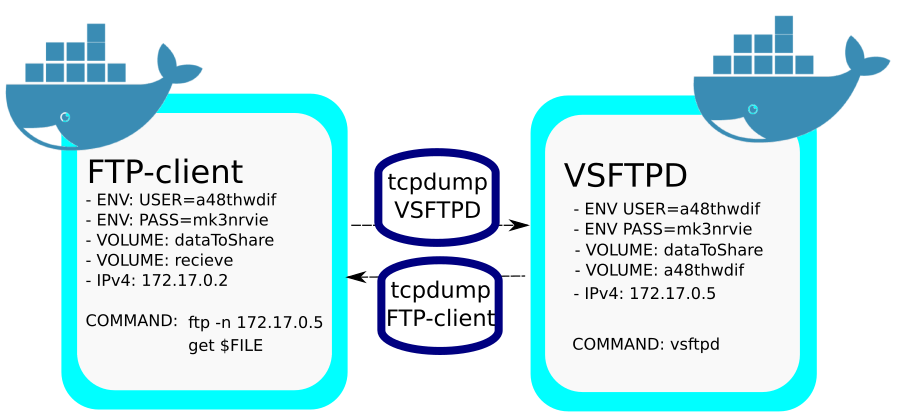
\includegraphics[width=0.49\textwidth]{images/ftp_new1.png}
%%\caption{Diagram of FTP scenario}
%%\end{figure}
%
%
%\subsection{Network-emulation}
%
%Describe the design of how the topology is generated before the data capture is started, and how the scenarios are launched and stopped during the data capture.
%\subsubsection{Topology generation}
%\dots \dots
%
%\dots \dots
%
%\dots \dots
%\subsubsection{Launch-script}
%
%\dots \dots
%
%\dots \dots
%
%\dots \dots
%
%\subsubsection{Dataset coalescence}\label{Sec:datasetcreation}
%\dots \dots
%
%\dots \dots
%
%\dots \dots
%\subsubsection{Activity timeline input}
%Here, we describe how the activity timeline in the launch script can come from unsophisticated distributions that we include, or from sophisticated 3rd party models such as Doppelganger. Since the modelling of computer activity is a field of ongoing research, it seems best to shift the responsibility for realistic models away by allowing this input. 
%
%\subsection{Microservice-emulation mode}
%
%\dots \dots
%
%\dots \dots
%
%\dots \dots


\section{Fidelity confirmation experiments}\label{Sec:Experiments}

This section is important to demonstrate that our data is valid and overcomes the difficulties entailed with synthetic data generation. Cordero et al. have proposed some more simple test that we can refer to first

\textcolor{red}{Question to be answered}: What requirements are there for the additional data, program logs and system logs, that we collect? Should we put less emphasise on these data sources in general if we are not able to perform these tests, and refer to them in future work? I am not aware of any papers that discuss these requirements in a similar way. 


\subsection{Data correctness tests}

This section is concerned with dataset defects, artifacts, or invalid data (inconsistent MTU etc.). These are very straightforward to test and should not take up much space. 


\subsection{Diversity tests}

These tests, also from Cordero et al. quantify diversity via the entropy of different quantities such as IP diversity, Time-to-Live, Maximum-segment-size, Window size, ToS. I think we should keep this relatively short and omit comparison to other datasets since this is already done by Cordero et al. 


\subsection{Structural dataset dimensionality}



Autoencoders are often used to compress non-deterministic, noisy data. Bahadur et al. have developed a procedure to estimate the ,,dimensionality'' (to be understood as the complexity) of a dataset using variational autoencoders. I believe we can transfer this concept to sequence compression and estimate the overall complexity of connection sequences in our framework with both real traffic captures and existing network intrusion datasets. 

Showing that our data is closer to real-world data would be a good test for "artificially predictable patterns", as described by Cordero et al., and go hand-in-hand with demonstrating the benefits of our framework for the training of deep-learning models. The importance of data that is less artificially predictable and closer to real-life traffic in terms of statistical variations lies in its suitability as a benchmark for detection rates, since less complex data is easier to train on and yields unrealistically high detection rates. 


%Measure structural richness of
%Also measure divergence across same activities (same activity and same port)
%Demonstrate benefit of structural richness
%Closer to reality



%\subsection{Reproducible scenarios}\label{Sec:deterministic}

%\dots \dots

%\dots \dots

%\dots \dots
%\begin{figure}
%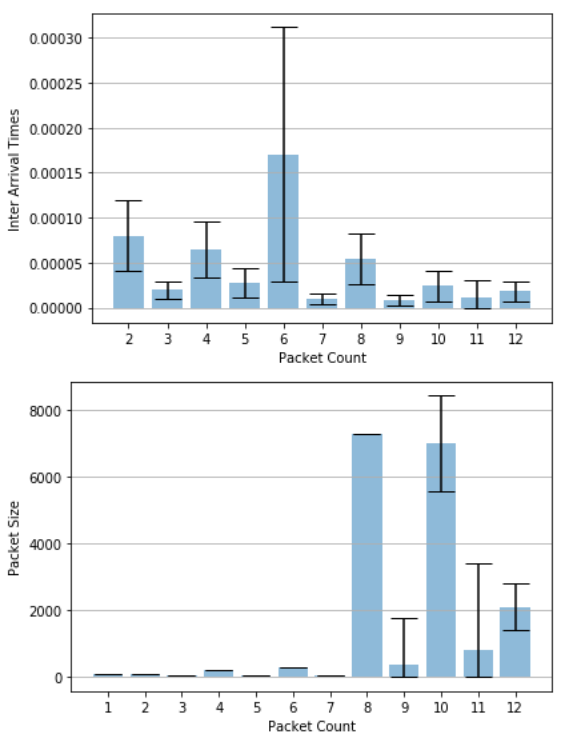
\includegraphics[width=0.45\textwidth]{images/combined3.png} % first figure itself
%\caption{Means of IATs \& packet sizes along with standard deviation bars for the first twelve packets in the Apache scenario.}
%\label{fig:size1}
%\end{figure}

 


% Need to edit these sections to provide a single context for both the artificial delays & classification

\subsection{Explorating Artificial Delays}

This section is already existing, we could potentially expand this. I think it is sufficient and analysing it more does not add much to the paper as the performance of TC netem is relatively well accepted. I think we could even move this section to the appendix.

%\begin{figure}
%\captionsetup{justification=centering}
%\centering
%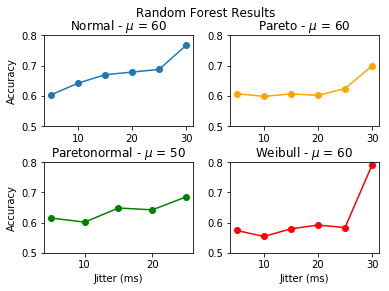
\includegraphics[width=0.45\textwidth]{images/1-plot_exp1.png}
%\caption{Results of Random Forest Classifier for a given distribution at the best performing delay mean $\mu$. Note that a score of .5 indicates total indistinguishability.}
%\label{Fig:rf_graph}
%\end{figure}
%
%
%
%\begin{table}[ht!]
%\begin{center}
%\begin{small}
%\begin{sc}
%\begin{tabular}{ccccc}
%\hline
%Distribution & Mean & Jitter & RF Accuracy\\
%\hline
%No Delays (Baseline) & 0 & 0ms & 0.8176 \\
%Constant Delay & 40ms & 0ms & 0.6730 \\
%Normal & 60ms & 5ms & 0.6028 \\
%Pareto & 60ms & 10ms & 0.5979 \\
%Paretonormal & 50ms & 10ms & 0.6015 \\
%Weibull & 60ms & 10ms & 0.5540 \\
%\hline
%\end{tabular}
%\end{sc}
%\end{small}
%\caption{Worst Random Forest accuracy rates for a given distribution}
%\label{tab:results-iat_rf}
%\end{center}
%\vskip -4mm
%\end{table}



\section{Use-cases}


\subsection{Benefits of ground-truth labels/dynamic dataset generation}
Possible title: \textbf{Dataset tuning to decrease false-positives}

Extensive ground-truth labels for our activities are arguably the most important contribution of the DetGen framework, so we should highlight their benefit most. Since ground-truth labels on attack data are existing in other datasets, we should emphasise the benefit of having labels for different activities. In my eyes, the most striking benefit arises for false-positive analysis, which we could then combine with showcasing the benefit of being able to generate different amounts of traffic for different activities.


\paragraph{Plan}
Implement the LSTM-model in the paper "An LSTM-Based Deep Learning Approach forClassifying Malicious Traffic at the Packet Level", train it on our data (both benign and attack traffic). Extract labels of traffic responsible for false-positives, show how much they are clustered around particular activities (potentially rare activities) compared to the overall traffic. Give potential reason for this. Generate a new dataset with increased amounts of the activities responsible for false positivies. Demonstrate that false-positives decrease.

\subsubsection{Benefits of structural richness}

Possible title: \textbf{Harder benchmarks}

As described above, the importance of data that is less artificially predictable and closer to real-life traffic in terms of statistical variations lies in its suitability as a benchmark for detection rates. In particular, we want to demonstrate that our data functions is a more difficult and realistic benchmark that is less prone to inflating detection rates than existing datasets, something that is often a point of criticism for models evaluated on synthetic data. 

To show that the training and detection is harder on our data, we could generate a dataset with similar attacks and services as the CICIDS-17 dataset, and train the above described LSTM model on both datasets. We could show that the training loss goes down more slowly on our data, as well as other metrics (increased validation loss --> overfitting etc.). We could then go ahead and show that the same attacks are detected easier by the same model in the CICIDS-17 data than in our data, concluding that it is a less realistic benchmark.

It would be good to also include a comparison with actual real-world traffic here to bolster our conclusion, but due to the lack of structured real-life datasets it is difficult to create a fair and scientific comparison. 

%\subsubsection{Show utility of tuning amount of rare events}

\subsection{Show utility of flexible topology}

This is another possibility to demonstrate that the flexibility provided through containerisation allows for better benchmarking and more in-depth evaluation.

Methods aiming at modelling network structures are an established method for botnet and pivoting detection. Even though the network topology is a crucial variable in their training, their evaluation is to my knowledge only done on single static datasets such as the LANL-15. 

My idea is that we generate about 10 datasets with different topologies, (especially different numbers of subnets and servers), and highlight the variation in prediction accuracy, i.e. the accuracy on one dataset is significantly higher/lower, and the average across the different datasets is a better indicator that eliminates the topology as a variable. We do not necessarily need to implement any attack traffic here since the modelling accuracy on benign traffic should be sufficiently quantifiable. 

A suitable candidate for the evaluation would be the paper "Link prediction in dynamic networks using randomdot product graphs", which comes from people at Imperial College that I know. The model tries to give a probability for each connection to appear in a network, in order to spot connections between unlikely pairs as anomalous behaviour. I could ask the people for the implemented model so we do not have to do it ourselves, or we could even have a chat with them.


%\begin{figure}%[ht!]
%\subfloat{%
% 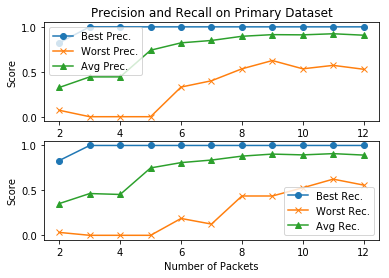
\includegraphics[width=0.4\textwidth]{images/bw_100_exp_3.png}}
%\subfloat{
% 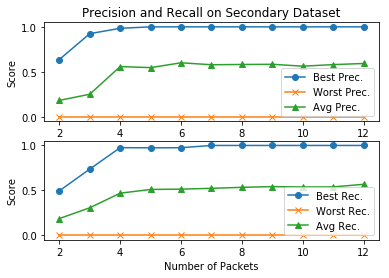
\includegraphics[width=0.4\textwidth]{images/bw_500_exp_3.png}}
%\caption{Results of Random Forest Classification on Primary dataset (Above) and Secondary dataset (Below)}
%\label{Fig:Primary}
%\end{figure}

\subsection{Customisable attack traffic by using metasploitable}

Rob and I discussed that by using a combination of a metasploit-attack container and a metasploitable-victim container, we could generate and embed a significantly larger number of attack traffic types more efficiently than we are currently. Since we can attach the metasploitable-container to the network interface of regular containers, we can embed the implemented vulnerabilities very easily in a given scenario. Furthermore, since both containers are well maintained, we can keep the attack catalogue up-to-date.

I think the best use-case is to showcase the process of adding a new type of attack to the dataset, embedding it in a proper way to a given scenario, generating data from it. We could additionally implement a corresponding detection method, but I think this would not demonstrate anything. 


\subsection{Simple use-case for the microservice mode?}
This use-case depends a lot on the state of the framework, but we could in principle show the benefits of the framework for the recently published model in "AppMine: Behavioral Analytics for Web Application Vulnerability Detection" on a more extensive dataset, since they only had very limited data available. 
\section{Conclusions}\label{Sec:Conclusion}



\subsection{Difficulties and limitations}


\subsection{Future work}



%Syslog logging driver
%add server to capture syslogs 

%https://docs.docker.com/config/containers/logging/syslog/


%We are grateful for our ongoing collaboration with our industry partners  on this topic area, who provided both ongoing support and guidance to this work. Discussions with them have helped reinforce the need for a better evaluation and understanding of the possibilities that new intelligent tools can provide.

%Full funding sources after currently blinded.

\bibliographystyle{abbrv}
 
\bibliography{DetGen_ext}

%\appendix


\end{document}
